%%%%%%%%%%%%%%%%%%%%%%%%%%%%%%%%%%%%%%%%%%%%%%%%%%%%%%%%%%%
%                                                         %
% CHAPTER 05:                                             %
% The virial theorem                                      %
%                                                         %
% This file is part of a BSc Thesis Project. See the      %
% LICENSE file for more information about licensing.      %
%                                                         %
% Author:     Matteo Seclì <secli.matteo@gmail.com>       %
% A.Y.:       2014/2015                                   %
% URL:        https://github.com/matteosecli/QMC          %
%                                                         %
%%%%%%%%%%%%%%%%%%%%%%%%%%%%%%%%%%%%%%%%%%%%%%%%%%%%%%%%%%%

\graphicspath{{Mainmatter/figures/PNG/}{Mainmatter/figures/PDF/}{Mainmatter/figures/}}

\chapter{The virial theorem}
\label{sec:virial}

The virial theorem states that the expectation value of the total kinetic energy $\Braket{T}$ is proportional to the expectation value of the total potential energy $\Braket{V}$. For a pure harmonic oscillator, this theorem is simply the theorem of the \emph{equipartition theorem}:
\begin{equation}
	\Braket{T} = \Braket{V}.
\end{equation}
This is quite easy to prove. Let's introduce the ladder operators
\begin{equation}
	\hat{a}=\frac{1}{\sqrt{2 \hbar \omega m}} \left( m \omega \hat{x}+ i \hat{p} \right)
	\qquad \text{and} \qquad
	\hat{a}^{\dagger}=\frac{1}{\sqrt{2 \hbar \omega m}} \left( m \omega \hat{x}- i \hat{p} \right)
\end{equation}
It can be shown that these operators act on the harmonic oscillator eigenstates such that
\begin{equation}
	\hat{a} \Ket{n} =\sqrt{n} \Ket{n-1}
	\quad \text{and} \quad 
	\hat{a}^{\dagger} \Ket{n} =\sqrt{n+1} \Ket{n+1},
\end{equation}
and we also have
\begin{equation}
	N\Ket{n} \doteqdot \hat{a}^{\dagger}\hat{a}\Ket{n} = n\Ket{n}.
\end{equation}

Using these properties, the calculation of the expected value of the potential energy is straightforward:
\begin{align}
	\Braket{n|\frac{1}{2}m\omega^2\hat{x}^2|n}
	&= \frac{1}{2}m\omega^2\Braket{n|\hat{x}^2|n} \\
	&= \frac{1}{2}\cancel{m}\omega^{\cancel{2}}\frac{\hbar}{2\cancel{m}\cancel{\omega}}\Braket{n|\left(\hat{a}^{\dagger}+\hat{a}\right)\left(\hat{a}+\hat{a}^{\dagger}\right)|n} \\
	&= \frac{\hbar\omega}{4} \left(\Braket{n|\hat{a}^{\dagger}\hat{a}^{\dagger}|n}+\Braket{n|\hat{a}\hat{a}^{\dagger}|n}+\Braket{n|\hat{a}^{\dagger}\hat{a}|n}+\Braket{n|\hat{a}\hat{a}|n}\right) \\
	&= \frac{\hbar\omega}{4} \left(\sqrt{n+2}\sqrt{n+1}\cancelto{0}{\Braket{n|n+2}}\right. \\
	&\left.+\Braket{n|\hat{N}+1|n}+\Braket{n|\hat{N}|n}+\sqrt{n}\sqrt{n-1}\cancelto{0}{\Braket{n|n-2}}\right) \\
	&= \frac{\hbar\omega}{4}((n+1)+n) = \frac{\hbar\omega}{4}(2n+1) \\
	&= \frac{\hbar\omega}{2}\left(n+\frac{1}{2}\right)
\end{align}
If we perform the same calculation for $\Braket{n|\frac{\hat{p}^2}{2m}|n}$ (the expected value of the kinetic energy) we will obtain the result, yielding
\begin{equation}
	\Braket{T} = \Braket{V}
\end{equation}
and
\begin{equation}
	\Braket{T}+\Braket{V} = \hbar\omega\left(n+\frac{1}{2}\right),
\end{equation}
that is the total energy of the harmonic oscillator, as expected.

Let's now graph the ratio $\Braket{T} / \Braket{V}$ for different values of $\omega$.

\section{The 2-electrons system}

We firstly computed $\Braket{T}$ and $\Braket{V}$ \emph{without} the electron-electron repulsion, to check our code. We chose $\omega=0.01,\,0.28,\,0.50,\,0.70,\,1.00$. The result -- completely expected -- is shown in Figure \ref{fig:virial_2e-norep}.
\begin{figure}[H]
	\centering
	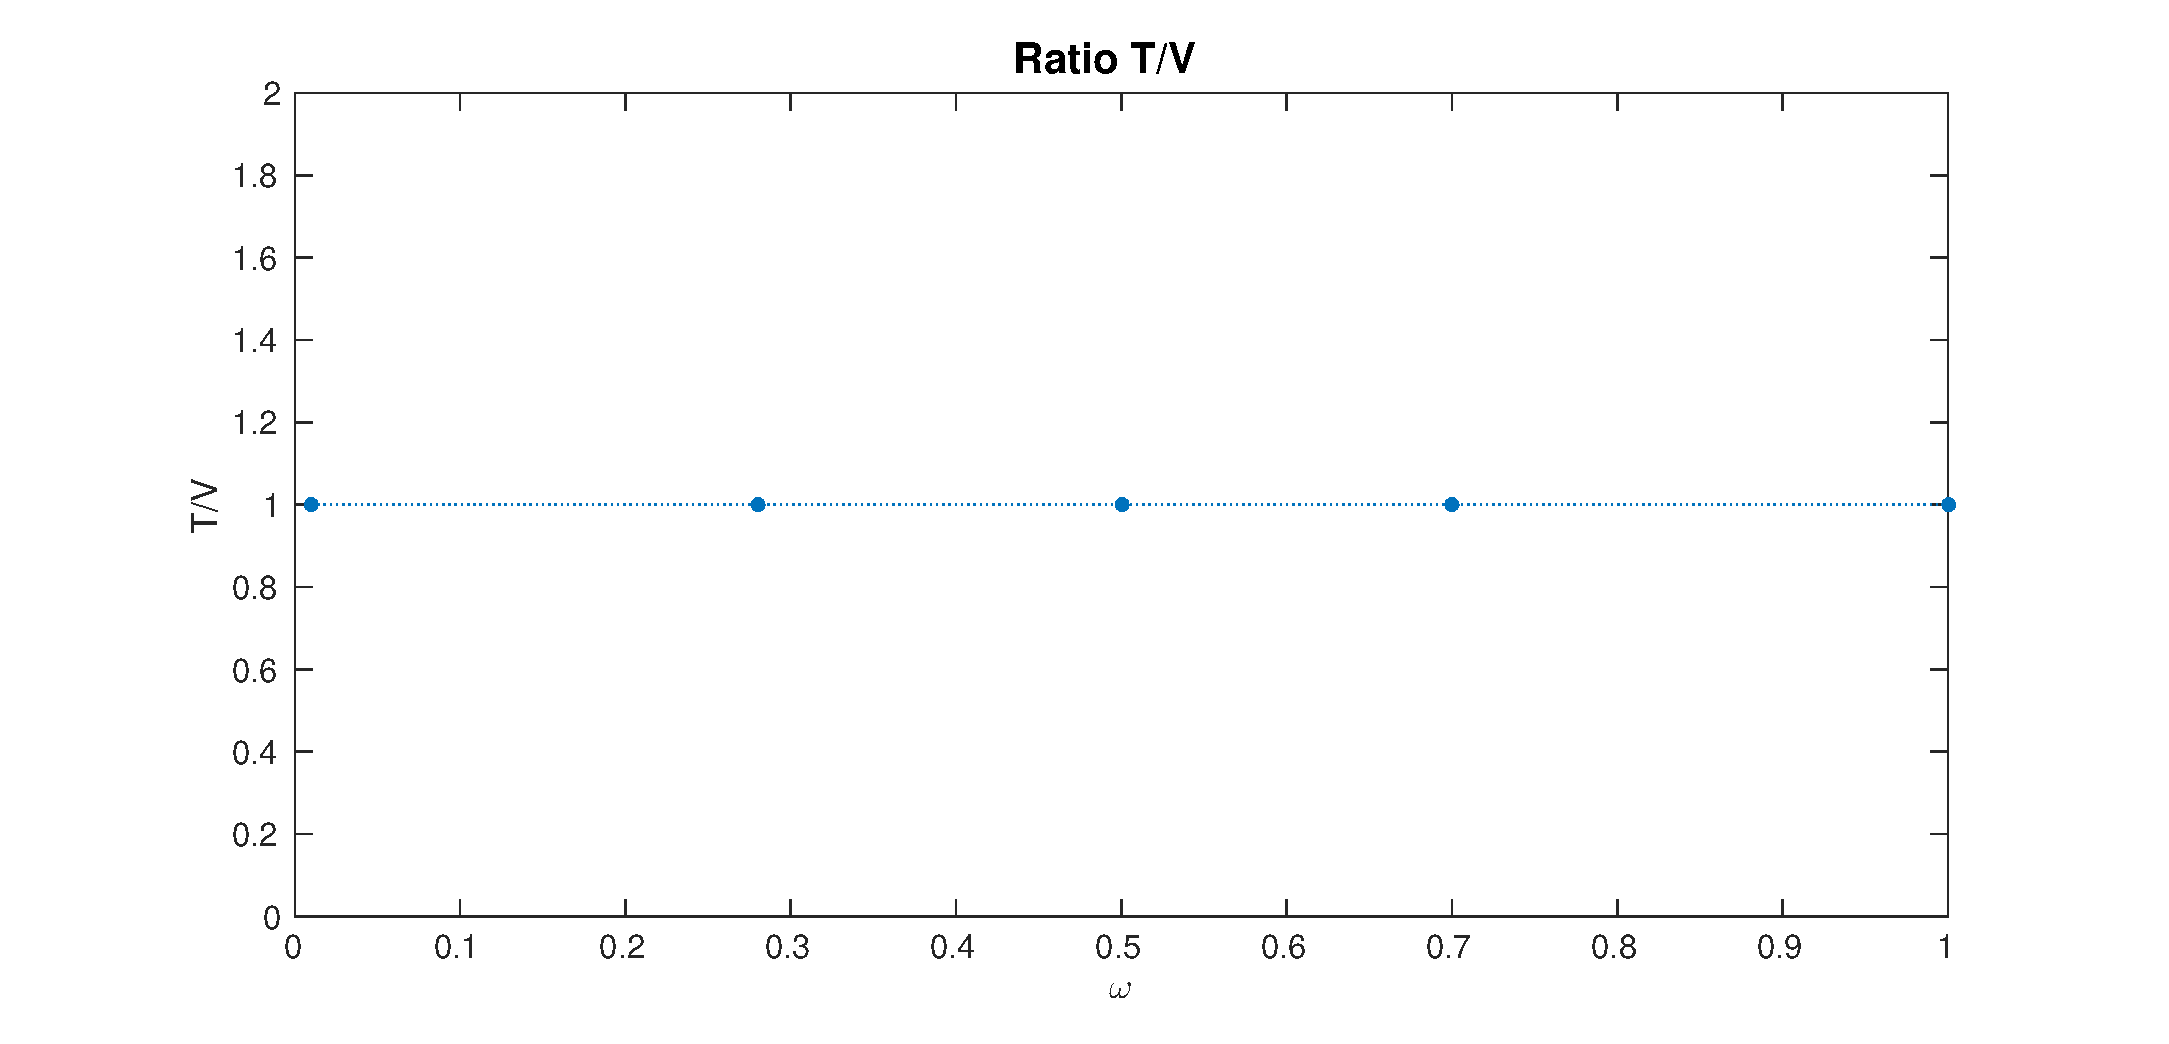
\includegraphics[width=\textwidth]{virial_2e-norep}
	\caption{The ratio $\Braket{T} / \Braket{V}$ for different values of $\omega$ and no electron-electron repulsion. The settings used are: importance sampling with $\Delta t = 0.1$, parallelization (8 threads), $\SI{1e7}{}$ Monte Carlo steps.}
	\label{fig:virial_2e-norep}
\end{figure}

After that, we added the electron-electron repulsion and we did again the calculations for the same $\omega$ values. The result, shown in Figure \ref{fig:virial_2e-rep}, is quite different.

\begin{figure}[H]
	\centering
	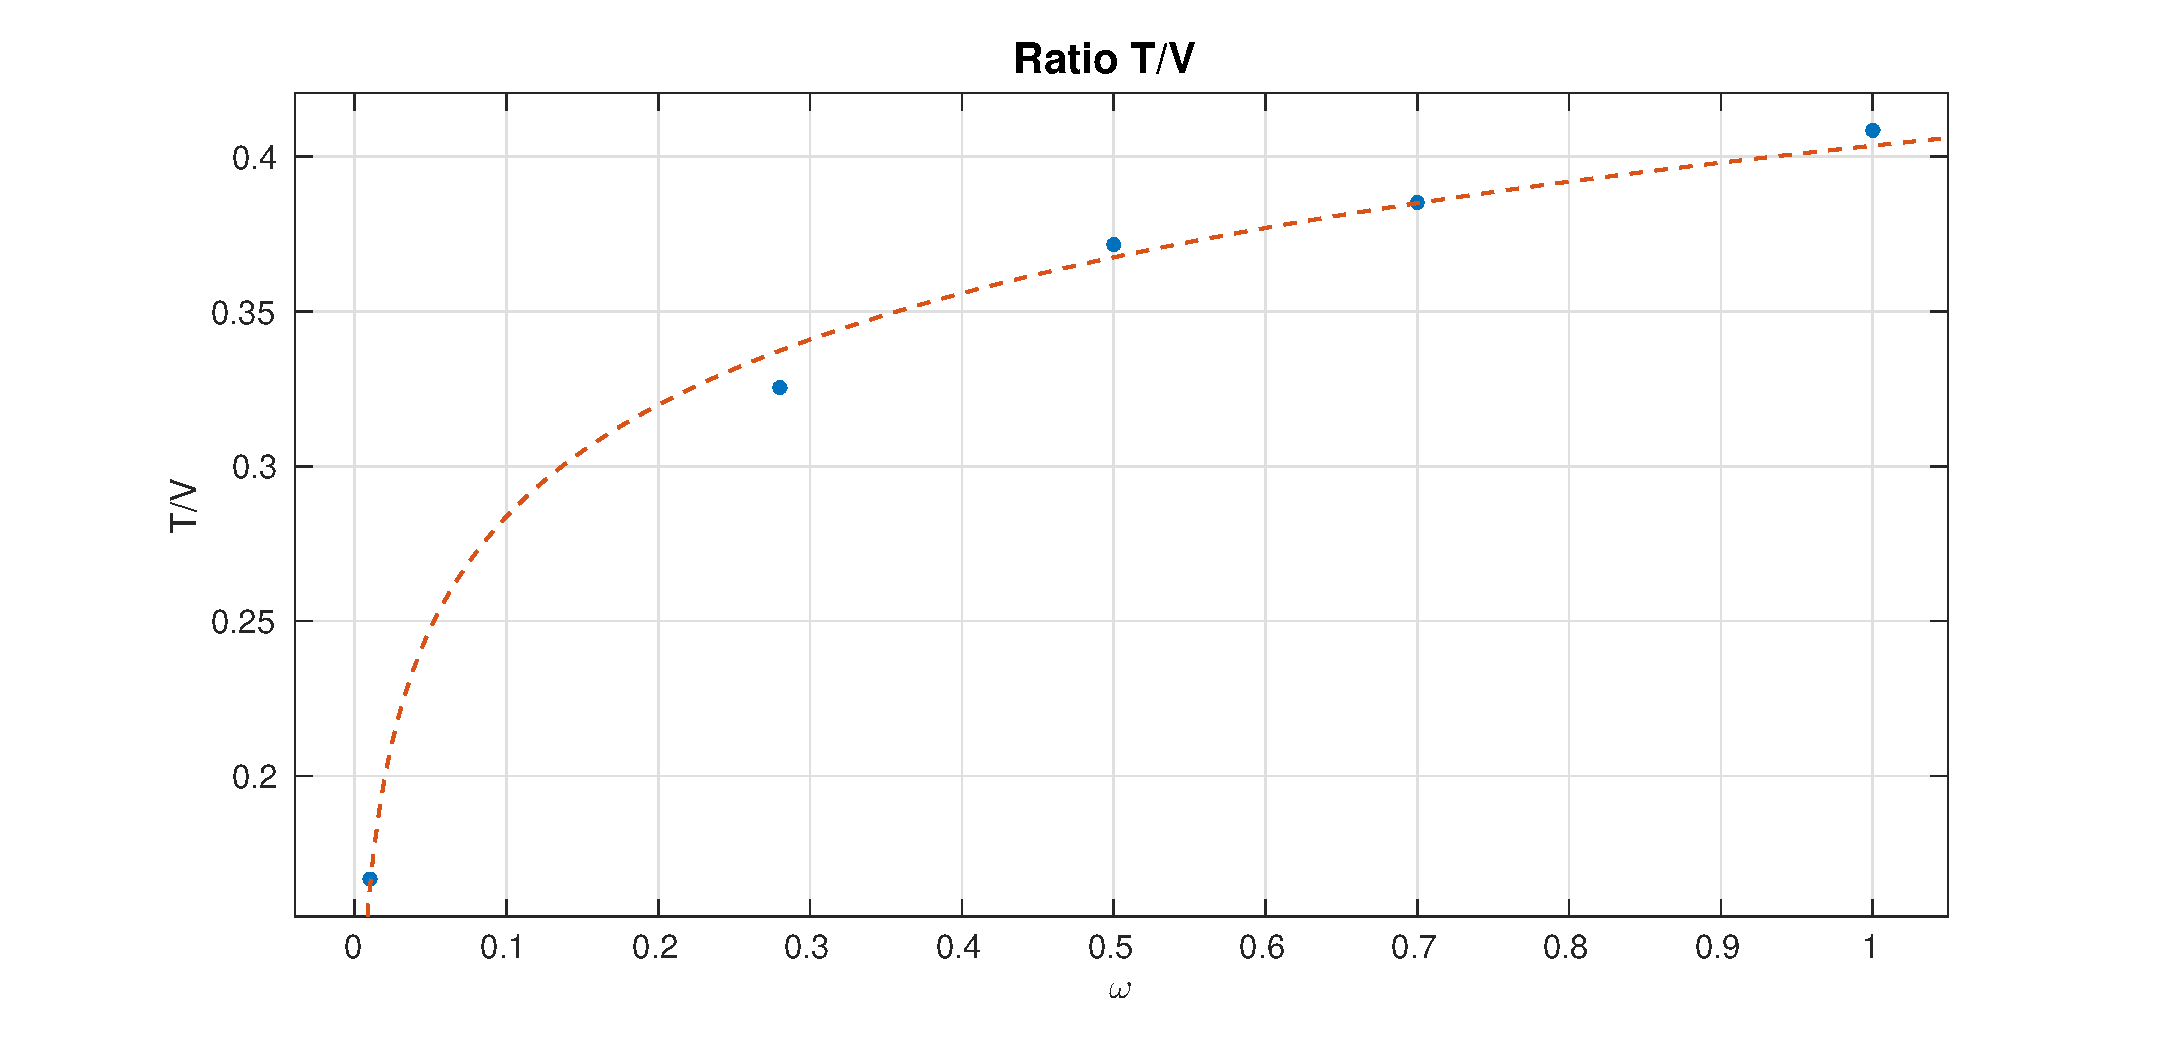
\includegraphics[width=\textwidth]{virial_2e-rep}
	\caption{The ratio $\Braket{T} / \Braket{V}$ for different values of $\omega$ with electron-electron repulsion. The settings used are: importance sampling with $\Delta t = 0.1$, Jastrow factor, parallelization (8 threads), $\SI{1e7}{}$ Monte Carlo steps. The fit is logarithmic.}
	\label{fig:virial_2e-rep}
\end{figure}

The dashed line is a fit of the type
\begin{equation}
	\frac{\Braket{T}}{\Braket{V}} = b\log(c\omega),
\end{equation}
which gives $b = \SI{0.052 \pm 0.007}{}$ and $c = \SI{2340 \pm 2021}{}$. We can't really say if the behaviour of our data is logarithmic without a theoretical basis and with just $5$ points; the purpose of the dashed line in Figure \ref{fig:virial_2e-rep} is just to show that our data is \emph{no way} linear. This is due to the presence of the repulsive force, that can be dominant or not.

In a very intuitive way, we can at least say that what we obtain is coherent with the physics of the system. For $\omega \gg 1$ the oscillator potential is dominant and the repulsion can be considered as a small perturbation, which means that we have more kinetic energy than potential energy ($T > V$). For $\omega \ll 1$, we almost have only a repulsion potential plus a small harmonic perturbation; in other words, $T < V$.

If one really wants to find an analytical relation for the ratio $\Braket{T} / \Braket{V}$ of this system, he should compute the two terms separately in a way similar to the one shown in Section \ref{sec:virial} and then take the ratio of them. Note that this is not always possible, since the necessary integrals could not be solved analytically.


\section{The 6-electrons system}

\begin{figure}[H]
	\centering
	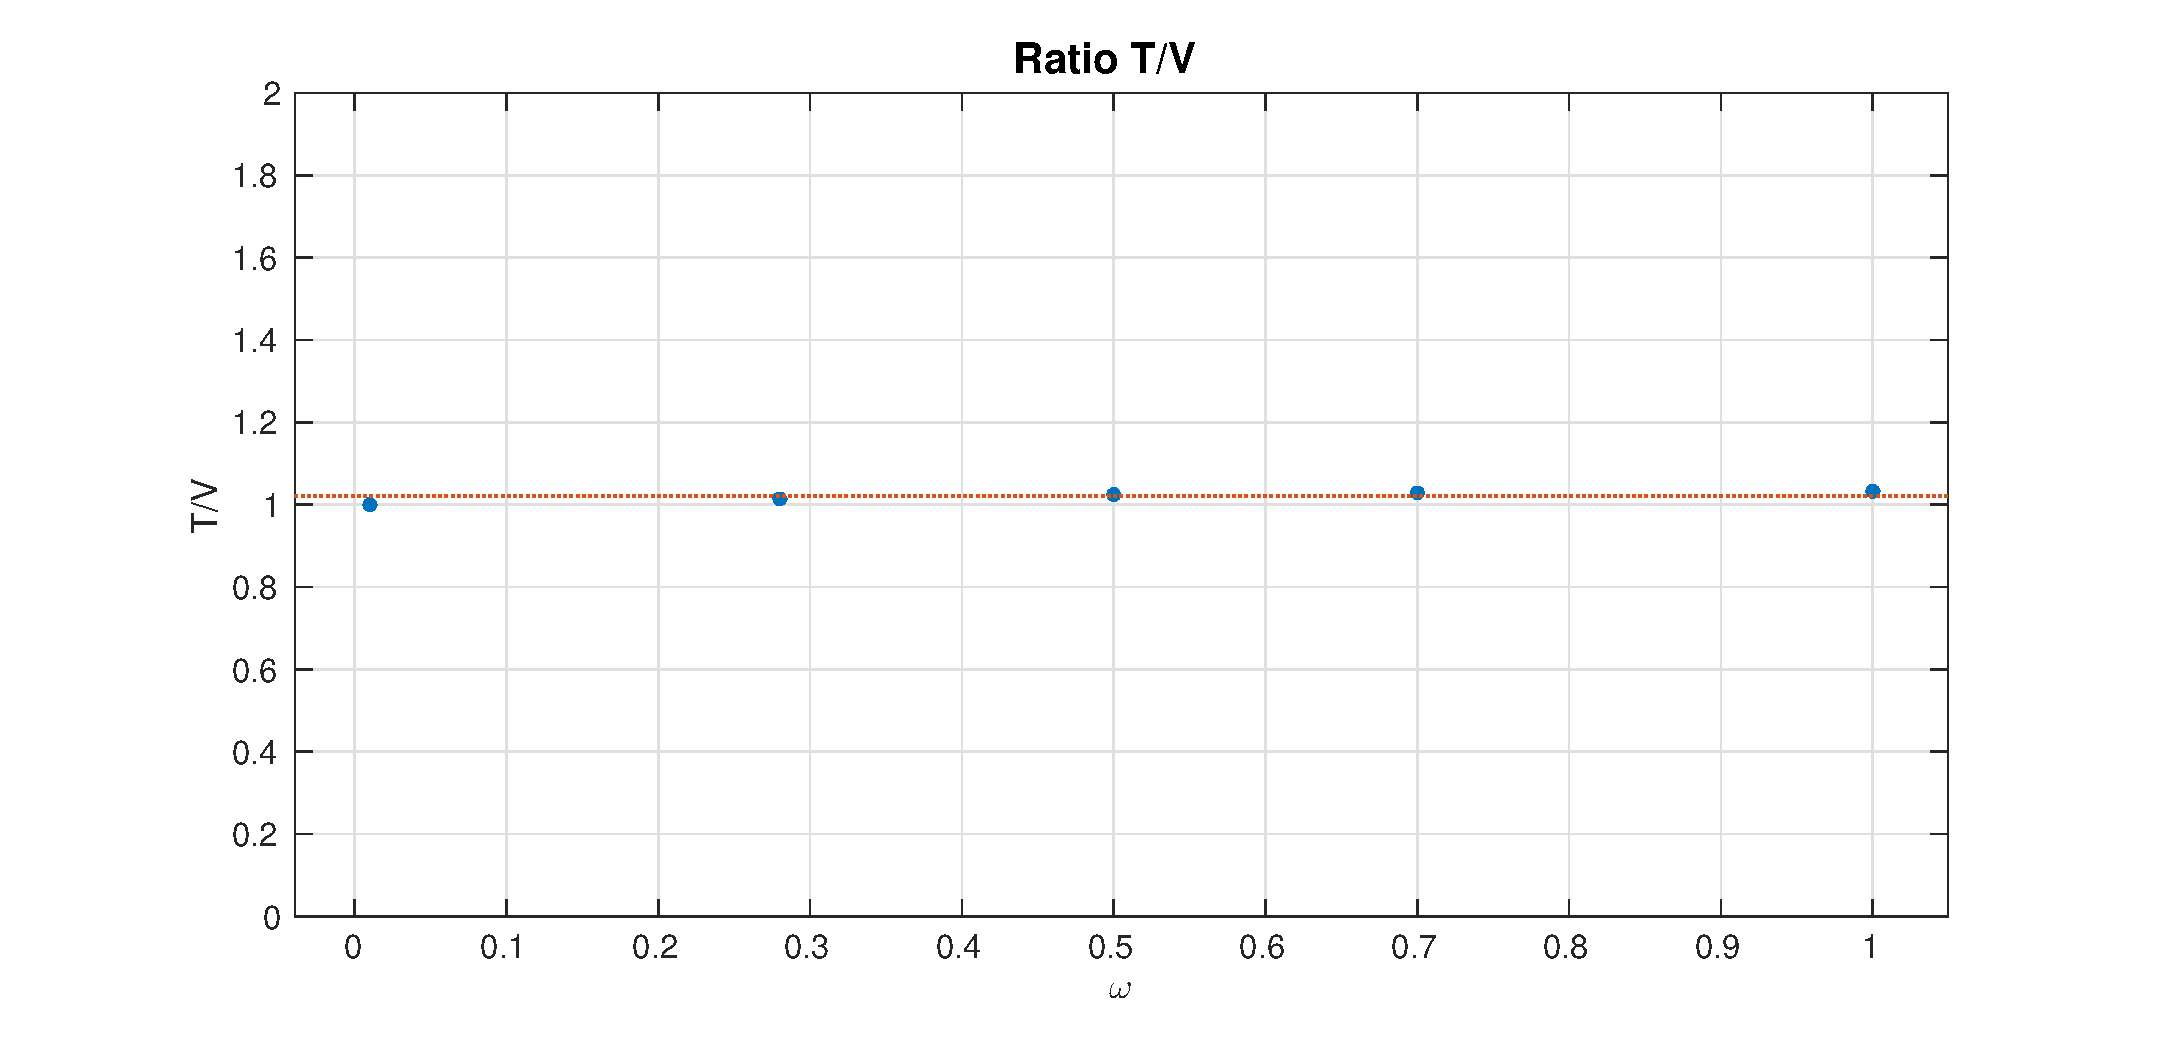
\includegraphics[width=\textwidth]{virial_6e-norep}
	\caption{The ratio $\Braket{T} / \Braket{V}$ for different values of $\omega$ and no electron-electron repulsion. The settings used are: importance sampling with $\Delta t = 0.1$, parallelization (8 threads), $\SI{1e6}{}$ Monte Carlo steps.
	A linear fit gives a ratio of $\SI{1.02 \pm 0.02}{}$, that is still compatible with the expected value $1$.}
	\label{fig:virial_6e-norep}
\end{figure}

\begin{figure}[H]
	\centering
	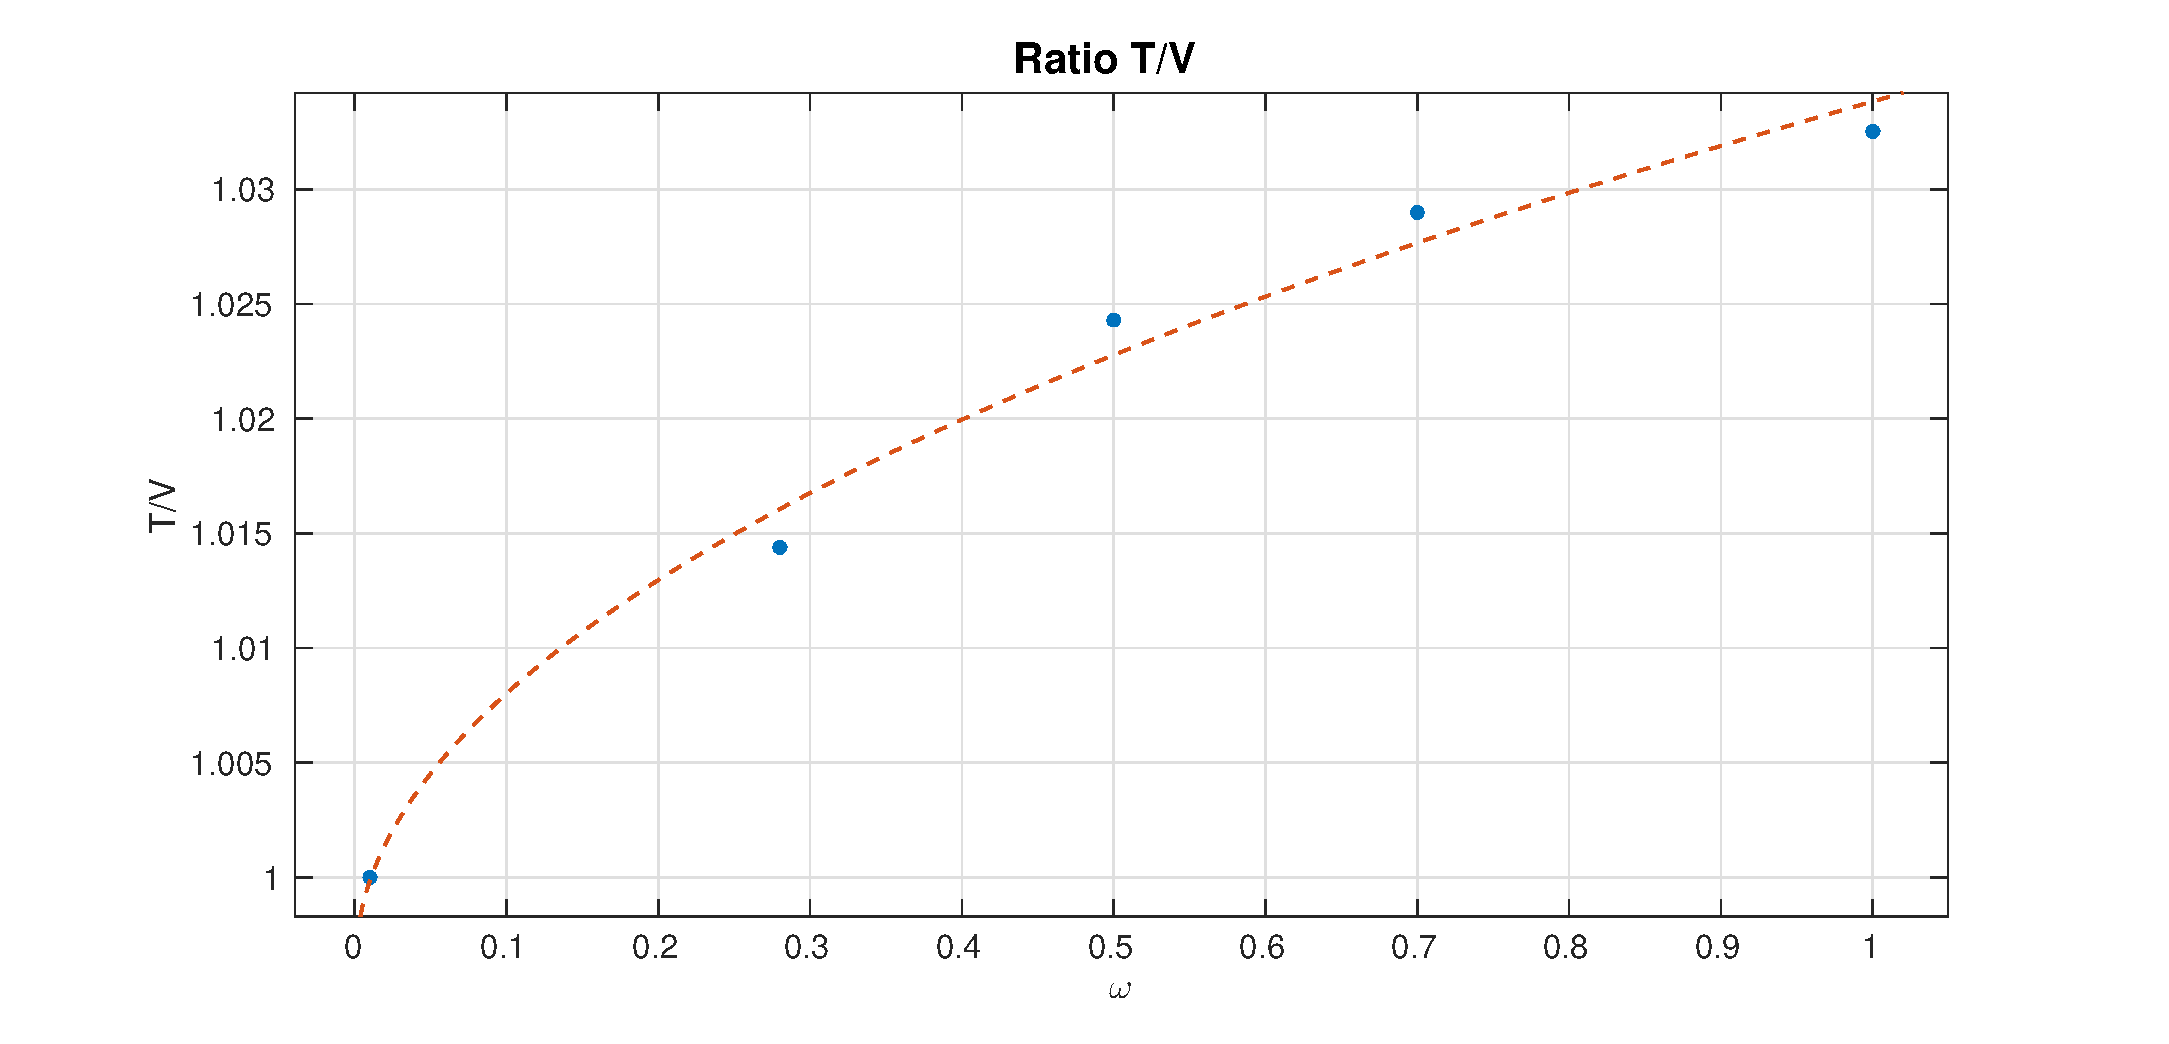
\includegraphics[width=\textwidth]{virial_6e-rep}
	\caption{The ratio $\Braket{T} / \Braket{V}$ for different values of $\omega$ with electron-electron repulsion. The settings used are: importance sampling with $\Delta t = 0.1$, Jastrow factor, parallelization (8 threads), $\SI{1e6}{}$ Monte Carlo steps. The fit is a square root.}
	\label{fig:virial_6e-rep}
\end{figure}

We did again the same calculations (with the same $\omega$ values) for $6$ electrons. This time, we don't obtain a perfect $1$ ratio for the non repulsive case (Figure \ref{fig:virial_6e-norep}); a linear fit gives $\SI{1.02 \pm 0.02}{}$, which is anyway still compatible with the expected value $1$. A possible explanation for this behaviour is that we are not using enough Monte Carlo steps; they are ten times less than the previous case, when we are dealing with a number of electrons that is three times more the 2-electrons case.

The discussion of what we obtain adding the electron-electron repulsion, shown in Figure \ref{fig:virial_6e-rep}, is the same as the 2-electrons case in the previous section. The fit (that \emph{is not} particularly indicative) is of the type
\begin{equation}
	\frac{\Braket{T}}{\Braket{V}} = b\sqrt{c\omega}+d,
\end{equation}
which gives $b = \SI{0.06 \pm 0.01}{}$, $c = \SI{0.416 \pm 0.001}{}$ and $d = \SI{1.00 \pm 0.01}{}$.